% lowell-prop.tex - Lowell Observatory DCT proposal template 
%   Last update 2016-07-08 by hroe@lowell.edu

% General Instructions:
%  
%   Places in the form that require user input are denoted by %%% in this tex
%   file.  Instructions for the sections immediately precede the %%% symbol.
%
%   If you are at a DCT partner institution:
%      - Please fill out at least the cover page portion of this template.
%      - Submit a PDF copy of it to your DCT partner representative, who 
%        will forward it to the DCT Scheduler (tac@lowell.edu)
%
%   Lowell Observatory Users:
%      - Abide by the length limits.
%      - Fill out the cover sheet completely.
%      - Keep in mind that you are writing for a non-specialist audience.
%      - Proposal deadline is listed in the Call for Proposals.
%      - Submit by sending the PDF of your proposal to tac@lowell.edu
%   
% Observer Information for DCT is available at:
%     https://jumar.lowell.edu/confluence/display/DCTIC/Observing+at+DCT
%
% Proposer Information for DCT is available at:
%     https://jumar.lowell.edu/confluence/display/DCTIC/DCT+Proposal+Information
% 
%   Questions/comments:  tac@lowell.edu

\documentclass{lowell-prop}

% Uncomment if using figures:
\usepackage{graphicx}

% Uncomment to provide options to siunitx for typesetting units (the class file
% already loads this package and provides the units in http://goo.gl/XzoK8H
% \usepackage[custom-options]{siunitx}
% *Do not* typeset microns as $\mu$m unless you are also expressing kilometers as $k$m.

% Use textgreek to use greek letters which are not math (such as in Hα)
%\usepackage{textgreek}

\begin{document}

% Which telescope(s) are you using?  
% Uncomment one, and only one, of the following lines.
% Note that currently this form is *only* used for DCT, but the following line 
% is here for future compatibility if other facilities are added.
\telescopes{DCT}	% for proposals using DCT only

% Give a descriptive title for the proposal in the \title command.
%
% Note that a title can be quite long; LaTeX will break the title into
% separate lines automatically.  If you wish to indicate line breaks
% yourself, do so with a `\\' command at the appropriate point in
% the title text.
%%%
\title{Mysteries of the universe solved: A superbly wrong title for a stupendously strong proposal for an absurdly large amount of telescope time}

% Investigator's (PI and CoI) information blocks.

% Please give the investigator's name, and email address. (The email address of
% the account used to send in the form will be used if you don't fill this in.)
% You must also indicate whether the investigator is a graduate student by
% putting a Y or an N inside the \gradstudent{} curly braces.
%
% Each member of the proposal team is identified with several bits of
% information.
%
%    \name{OBSERVER NAME}
%    \affil{AFFILIATION}
%    \address{POSTAL ADDRESS}
%    \emailaddress{EMAIL ADDRESS}
%    \phone{TELEPHONE NUMBER}
%    \fax{FAX NUMBER}
%    \gradstudent{Y or N}
%    \undergradstudent{Y or N}
%
% Please note that the fax number does not print on the form at this
% time; this is intentional.  We can get your fax number from the
% electronic file if we really have to.
%
% DO NOT remove the \begin{PI} and \end{PI} or the \begin{CoI} and
% \end{CoI} lines.
%
% It is OK to remove unused CoI blocks or add additional CoI blocks as needed.

%%%
\begin{PI}
\name{J. X. Doe}			% REQUIRED
\affiliation{Lowell Observatory}		% REQUIRED
\emailaddress{jxd@lowell.edu}		% REQUIRED
\end{PI}

\begin{CoI}
\name{J. Y. Doe}			% REQUIRED
\affiliation{Lowell Observatory}		% REQUIRED
\emailaddress{jyd@lowell.edu}		% REQUIRED
\end{CoI}

\begin{CoI}
\name{J. Z. Doe}			% REQUIRED
\affiliation{Lowell Observatory}		% REQUIRED
\emailaddress{jzd@lowell.edu}		% REQUIRED
\end{CoI}

\begin{CoI}
\name{J. A. Doe}			% REQUIRED
\affiliation{Lowell Observatory}		% REQUIRED
\emailaddress{jad@lowell.edu}		% REQUIRED
\end{CoI}

\begin{CoI}
\name{J. B. Doe}			% REQUIRED
\affiliation{Lowell Observatory}		% REQUIRED
\emailaddress{jbd@lowell.edu}		% REQUIRED
\end{CoI}

%\begin{CoI}
%\name{J. C. Doe}			% REQUIRED
%\affiliation{Lowell Observatory}		% REQUIRED
%\emailaddress{jcd@lowell.edu}		% REQUIRED
%\end{CoI}

%\begin{CoI}
%\name{}			% REQUIRED
%\affiliation{}		% REQUIRED
%\emailaddress{}		% REQUIRED
%\end{CoI}


% As of 2016Q4, DCT observing proposals do not include an abstract.


% Indicate whether this proposal is part of Masters or PhD thesis work by
% uncommenting the following \thesis block.  Explain in the Scientific 
% Justification section how this proposal the proposed observations
% are required for the thesis.

%%%
%\thesis{}  % uncomment this line if this proposal is part of a Masters or PhD thesis.

% List the details of the observing runs being requested.  
% The parameters for each run are segregated
% between \begin{obsrun} and \end{obsrun} lines.  Please be sure
% that the information is isolated properly for each run.
% Up to a total of 10 observing runs are allowed on the form.
% Up to 3 observing runs will be shown on the primary cover page. 
% Observing runs #4 to #10 will be shown on the overflow cover page.
% If the information doesn't quite fit, try preceding it with a
% \small, e.g. \instrument{\small Lengthy description of instrument}
%
%   \telescope{}	For example, \telescope{DCT}
%   \instrument{}	For example, \instrument{LMI: UBVRI, H\textalpha-on,H\textalpha-off; 
%                                                OptiNIRSpec Spectrograph}
%   \numfirsthalfnights{} For exmaple, \numfirsthalfnights{3}
%   \numsecondhalfnights{} For exmaple, \numsecondhalfnights{3}
%   \moonbrightness{}	For example, \moonbrightness{D}
%   \optimaldates{}	For example, \optimaldates{Sept--Nov}
%   \acceptabledates{}	For example, \acceptabledates{Sept -- mid-Dec}
%   \remoteobserving{}  Either Y or N, if remote observing support is requested.  
%
% \moonbrightness should specify the maximum acceptable mean moon brightness
% using the following codes:
%     D = <=25%  (Dark)
%     G = <=70%  (Gray)
%     B = >70%   (Bright)
% Mean moon brightness is calculated as the mean fractional illumination of the
% moon (zero if below the horizon) outside of nautical twilight
%
% \optimaldates should contain the range of OPTIMAL dates 
%
% \acceptabledates should give the range of ACCEPTABLE dates (i.e., you
% would not accept time outside those limits).
%
% \wholenightsrequired is Y or N. (or "-" for ToO). In general scheduling will 
% attempt to schedule as whole nights if possible. However, programs may be
% split to half-nights as needed to make the schedule work. If there is a 
% reason you cannot accept half-nights, then enter "Y" and justify in your 
% Technical Justification section.
%
% When requesting specific nights, please specify them in local MST & explicitly
% state what you are are requesting.  
%   e.g.
% "We are requesting the second half of 27-Feb (MST)." 
%   -> is requesting the 2nd half of the night that started on 27-Feb (MST)
%      (although the actual time in UT is 28-Feb)
% (If concerned, you may specify in both UT & MST, e.g. "The occultation occurs
%  between 10:15 and 11:45 on 28-Feb (UT), therefore we are requesting the
%  second half of 27-Feb (MST).")
%
% For Target of Opportunity (ToO) program, use the alternate \begin{ToOrun} block.
% Additional details of the requested ToO observations should be placed in
% Technical Justification.

% DO NOT remove the \begin{obsrun} and \end{obsrun} blocks

%%%
\begin{obsrun}
\telescope{DCT}
\instrument{LMI: UBVRI}
\numfirsthalfnights{3}
\numsecondhalfnights{2}
\moonbrightness{D}
\optimaldates{Feb -- Mar}
\acceptabledates{Jan -- Mar, May-Jun}
\remoteobserving{N}
\wholenightsrequired{N}
\end{obsrun}

\begin{ToOrun}
\telescope{DCT}
\instrument{LMI}
\moonbrightness{any}  % Typically "any" for most ToO programs, but can also be D,G,B following above codes
\ToOtype{Rapid}   %  "Rapid" (10 minute response time) or "Slow" (30 minute response time)
\totalhours{5.0}
\end{ToOrun}


%\begin{obsrun}
%\telescope{DCT}
%\instrument{}
%\numfirsthalfnights{}
%\numsecondhalfnights{}
%\moonbrightness{}
%\optimaldates{}
%\acceptabledates{}
%\remoteobserving{}
%\wholenightsrequired{}
%\end{obsrun}

%\begin{ToOrun}
%\telescope{DCT}
%\instrument{}
%\moonbrightness{any}  % Typically "any" for most ToO programs, but can also be D,G,B following above codes
%\ToOtype{}   %  "Rapid" (10 minute response time) or "Slow" (30 minute response time)
%\totalhours{}
%\end{ToOrun}

% You may supply more obsrun blocks. Three will be displayed on the cover page
% and the remainder will be placed on an additional overflow cover page.

% do not delete or comment out the following \printCoverPageObsRuns{} block
\printCoverPageObsRuns{}

% List the people who will be performing the observations, either on-site or
% remotely. Highlight if any observers are new & in need of training.
% Note that remote observers must have observed at least once on-site
% with the scheduled instrument to be qualified.

%%%
\ObserversAndQualifications{Jane Z.\ Doe will do the 29-Jan (MST) observing run \& is a new observer.  \newline
Jane X.\ Doe has previously used LMI \& will do the ToO observations.}

% If you are requesting Time Critical Observation (TCO) status for some aspect
% of your observations, please uncomment the following \TimeCriticalObs{} block
% and briefly summarize the times/dates of the TCO request in one line or less, 
% e.g.:  "TCO status requested for night of 29-Jan (MST)."  
% Additional justification for the TCO request can be given in the Technical 
% Justification section.

%%%
\TimeCriticalObs{TCO status requested for night of 29-Jan (MST).}

% You may also offer additional specifics of requests regarding dates, instruments,
% cadence of observations, etc etc. in the following \MoreObsrunInfo{} block.
% Leave this next line commented out unless you are using it.

%%%
%\MoreObsrunInfo{Place any additional info regarding dates, instruments, cadence of observations, etc. here. Will be placed on overflow cover page, so can be longer than a few lines.}

% Other scheduling comments, such as dates (local MST) you cannot use 
% for non-astronomical reasons, go in \unusabledates
% If there are dates that you cannot use for non-astronomical reasons,
% please give the dates by filling in the curly braces in \unusabledates{}.
% Please explain briefly; \unusabledates is limited to a few lines.

%%%
\unusabledates{
January 24-26, attending conference  Donec euismod egestas ligula ut semper. Pellentesque ultricies metus sit amet laoreet dictum. Pellentesque efficitur leo id orci condimentum lacinia. Vestibulum egestas fermentum dictum. Vestibulum velit lorem, luctus nec sodales eget, rutrum id lorem. git status
}

% Don't edit or comment out the following line containing \OverflowFromCoverPage{}
% This line will create an additional page if needed to list more CoIs or more observing runs
\OverflowFromCoverPage{}

% In the following "essay question" sections, the delimiting pieces of
% markup (\scienceJustification, \feasibility, etc.) act as LaTeX \section*{}
% commands.  If the author wanted to have numbered subsections within
% any of these (as per this sample), LaTeX's \subsection could be used.

% Give the scientific justification for the experiment.
% This section should consist of paragraphs of text (and may include
% figures) that follow the \scienceJustification line.
% Be sure to include overall significance to astronomy.

% The Science Justification section is limited to one page of text and figure(s); 
% References may appear on a second page. 
% You may use your 1 page of Science Justification as you wish, but do not alter 
% default line spacing, margins, font size. 
% Most proposals should consist of no more than ~300 words of text and a figure. 
% Figures should be legible and not too small. Write for a general scientific audience.

% In order to include a plot, you should use the LaTeX "figure"
% environment with the graphicx package. For example:
%
% \begin{figure}
%     \includegraphics[scale=0.3]{fig} % for fig.pdf, fig.png or fig.eps
%     \caption{Sample Figure showing important results.\label{fig:name}
% \end{figure}

% If you are absolutely convinced you understand and are obeying the page limit of the 
% Scientific Justification section, you may uncomment the following flag, which will 
% remove the instructions for this section from the PDF and buy you a little more space.
% But, if you do that *and* break the page limit, a pox will be cast upon you.
% And, if you break the page limit and leave the instructions in, then you're just not
% paying attention.
% \removeScienceJustificationInstructions

%%%
\scienceJustification


Lorem ipsum dolor sit amet 10$\fdg$3, not 9$\farcm$1 nor 22$\farcs$32, consectetur adipiscing elit. Etiam vitae felis lectus 2.12~$\micron$. Nulla eu malesuada arcu. Aliquam a arcu in orci semper venenatis sed non purus. Pellentesque tempus nibh dolor. Donec eros lorem, gravida quis euismod eu, tempus sit amet neque. Maecenas tempus ex fermentum purus maximus porttitor. Class aptent taciti sociosqu ad litora torquent per conubia nostra, per inceptos himenaeos. Sed nec metus suscipit metus ultricies fringilla. Pellentesque habitant morbi tristique senectus et netus et malesuada fames ac turpis egestas. Praesent id viverra eros.

Donec euismod egestas ligula ut semper. Pellentesque ultricies metus sit amet laoreet dictum. Pellentesque efficitur leo id orci condimentum lacinia. Vestibulum egestas fermentum dictum. Vestibulum velit lorem, luctus nec sodales eget, rutrum id lorem. In convallis posuere ligula, ac interdum tortor lacinia sit amet. Aenean pulvinar rutrum velit, quis facilisis magna porta a. Praesent et est ac massa posuere lobortis. Proin hendrerit eros ac tincidunt luctus. Maecenas mollis dolor velit, ut iaculis sem efficitur eget. Duis mattis mollis maximus. In vulputate blandit nisl quis pulvinar. Morbi imperdiet ultrices sodales. Nam gravida varius urna, quis dignissim mi dignissim eu. Etiam justo mi, facilisis ac eleifend sagittis, euismod id arcu. Praesent elementum finibus diam, vitae gravida risus lacinia et.

Morbi mattis non purus at pulvinar. Nullam sollicitudin pretium mi id interdum. Sed eget neque diam. Nam nec arcu at orci luctus efficitur. In a ante rhoncus, scelerisque purus quis, rhoncus nibh. Nunc eget laoreet diam. Integer a fermentum nibh. Fusce luctus fermentum odio, vitae consequat neque fermentum facilisis. Morbi vehicula nec ligula eu rhoncus. Donec in sapien vitae risus condimentum rutrum vel non nisl. Suspendisse potenti. Class aptent taciti sociosqu ad litora torquent per conubia nostra, per inceptos himenaeos. Aliquam imperdiet dignissim neque, in varius lacus dictum aliquet. Ut quis sollicitudin ipsum.

 \begin{figure}[h]
   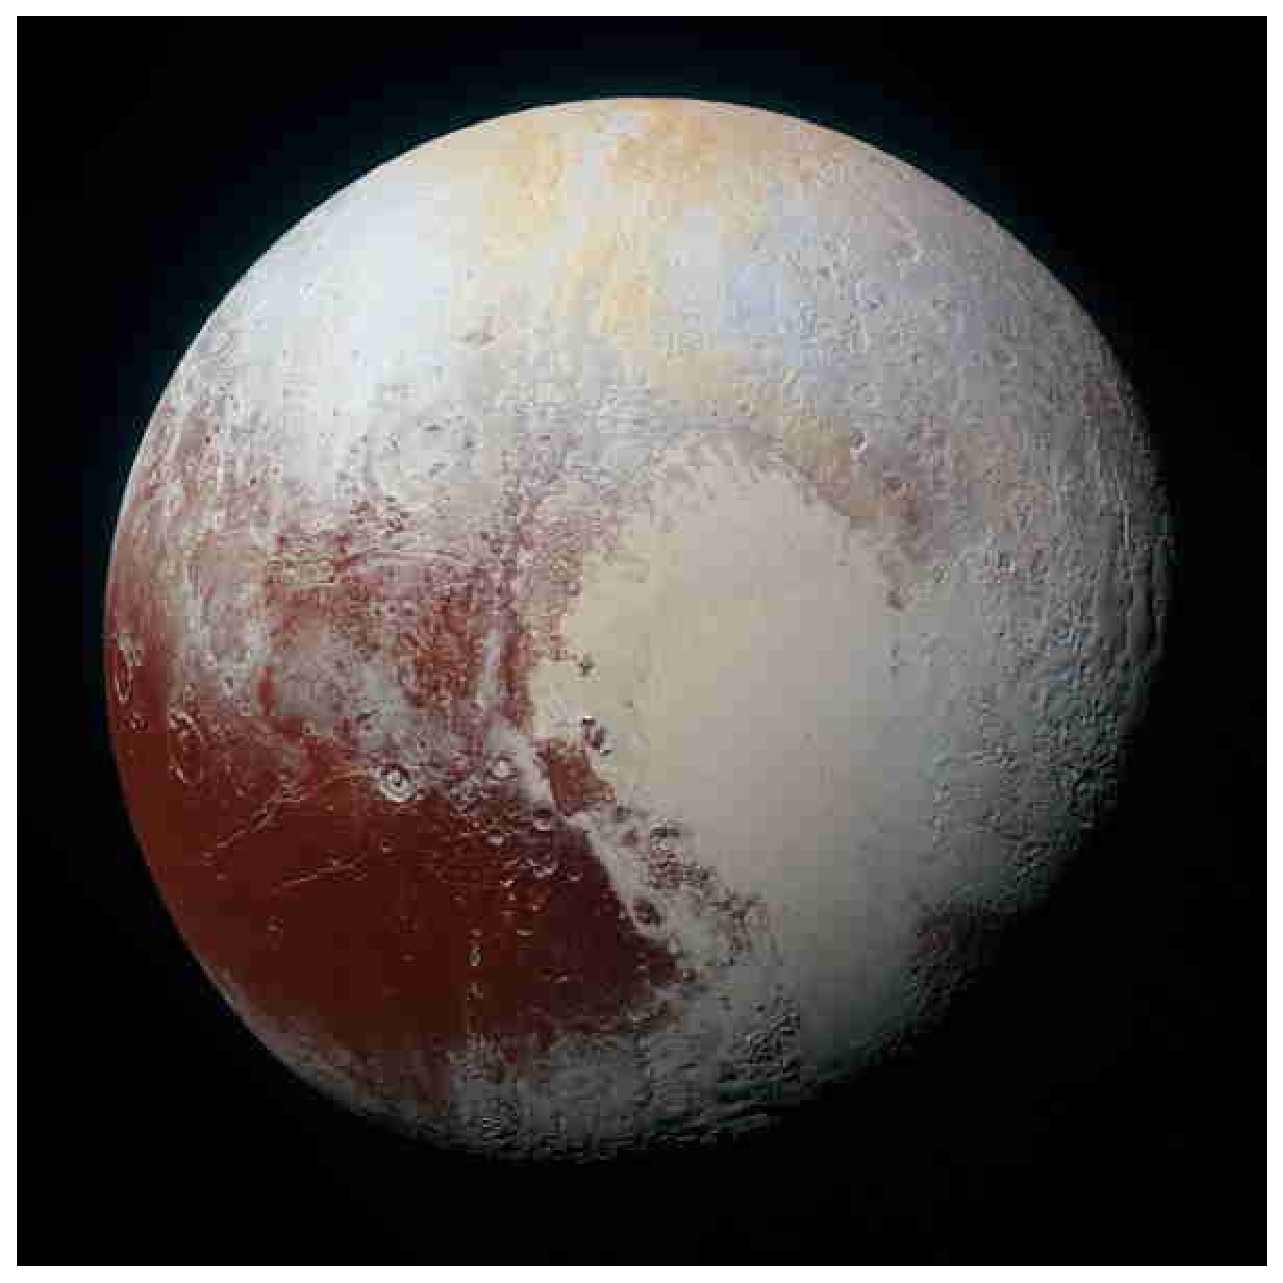
\includegraphics[width=0.5\textwidth]{pluto-small.eps} % for fig.pdf, fig.png or fig.eps
      \caption{We predict Pluto will look like this.}\label{fig:name}
 \end{figure}

% Example references section:

\bibliographystyle{abbrv}
\begin{thebibliography}{99}
\bibitem{1930PASP...42..351B} Burwell, C.~G.\ 1930.\ Note on 
Lines in the Red Region of the Spectra of Dwarf Stars of Classes K and M.\ 
Publications of the Astronomical Society of the Pacific 42, 351. 

\bibitem{1930Obs....53..342E} Eddington, A.~S.\ 1930.\ The 
connection of mass with luminosity for stars.\ The Observatory 53, 342-344. 

\bibitem{1930PASP...42..355J} Jones, R.~B.\ 1930.\ The Orbit 
of the Spectroscopic Binary {$\epsilon$} Librae.\ Publications of the 
Astronomical Society of the Pacific 42, 355. 

\bibitem{1930PASP...42..346M} Moore, C.~E.\ 1930.\ The 
Presence of Ionized Lutecium in the Sun.\ Publications of the Astronomical 
Society of the Pacific 42, 346. 

\bibitem{1930PASP...42..330M} Moore, J.~H., Menzel, 
D.~H.\ 1930.\ The Rotation of Uranus.\ Publications of the Astronomical 
Society of the Pacific 42, 330. 

\bibitem{1930PASP...42..350N} Nicholson, S.~B., 
Mayall, N.~U.\ 1930.\ The Probable Value of the Mass of Pluto.\ 
Publications of the Astronomical Society of the Pacific 42, 350. 

\bibitem{1930Natur.126..993V} Vowles, H.~P.\ 1930.\ Persian 
Science and Jundishapur..\ Nature 126, 993-994. 

\end{thebibliography}

% Provide additional details of your observing request.
%
% This section should consist of paragraphs of text only (no figures)
% that follow the \observingRequest line.
%
% Limit to one page of text excluding target list. 
% 
% Justify the amount of time requested as well as the specific 
% instrument(s), configuration, & lunar phase. List objects, coordinates, 
% magnitude/surface brightness, desired S/N, wavelength coverage & 
% resolution. Justify any request for Time Critical Observation (TCO) 
% status. Justify & explain details of any Target of Opportunity (ToO) 
% request. If you require whole (vs. half) nights, explain why.
%%%
\observingRequest 

Proin in mollis purus. Nullam erat nunc, elementum nec sollicitudin sed, tincidunt eget sapien. Donec in sem eu odio luctus commodo. Integer accumsan risus ut laoreet vulputate. Aenean quis tempor nunc. Suspendisse pretium ornare vestibulum. Aliquam sollicitudin ac est ac sodales. Ut euismod purus vitae ipsum blandit, vitae semper libero ultrices. Etiam posuere vel dolor ac tempor. Curabitur dapibus pulvinar feugiat. Vivamus nec pellentesque ex. In maximus, nisi congue efficitur tempus, arcu risus eleifend orci, eu facilisis mi sapien non velit. Nam pharetra mollis diam, eu egestas ligula sagittis ac. Cras in nisl accumsan, elementum neque id, aliquet ante. Nam tristique purus sit amet tellus pretium, non fermentum enim dignissim. Nulla facilisis cursus auctor.

Aenean sit amet ornare massa. Integer porta magna aliquet eros tempus, non egestas lorem vehicula. Vivamus sit amet ultrices justo, non euismod nisl. In sed eleifend justo. Sed in purus mi. Sed ac odio imperdiet, tempor elit eget, mollis diam. Phasellus nisl mi, laoreet eu ultrices id, tincidunt quis mauris. In in felis in nisl molestie lacinia vitae eget massa. Nullam tempus lorem velit, eu tincidunt tortor posuere eu. Curabitur malesuada ipsum et maximus lacinia. Donec nibh mauris, lacinia in mi id, vehicula mattis massa. Fusce iaculis in nulla ut luctus. Donec eu eleifend dui. Donec id erat in lacus sodales euismod eu eget augue.

\clearpage

% Fill in the following table with your target list

%%%

\begin{center}
{\bf Target List} \\[2em]
\begin{tabular}{l l l l l} 
\hline\hline 
&   &   &Integration&  \\
Object & Coordinates & Mag & Time & Comments \\ [0.5ex] 
\hline 
Some star & 15$^h$ 30$^m$, $-4^{\circ}$ & K=7.5 & 1.5 hr & Main program object, etc. \\
   &   &   &   & \\
   &   &   &   & \\
   &   &   &   & \\
   &   &   &   & \\  [1ex] 
\hline 
\end{tabular}
\end{center}


\end{document}

